\section{Ejercicio 5}
\label{sec:ej5}

Este ejercicio pedía experimentar con el scheduler round robin desarrollado en
el punto anterior. Para ello, primero se generó un lote con 3 tareas
\texttt{TaskCPU} de 70 ciclos y 2 \texttt{TaskConsola} con 3 llamadas
bloqueantes de duración 3. Luego se realizaron las siguientes pruebas donde lo
que se fue modificando fue la cantidad de núcleos y el quantum asignado a cada
uno.

En la Figura \ref{fig:ej1_3n} se configuró el simulador para utilzar 3 núcleos
con quantums de 2, 10 y 30. Se puede observar cómo al disponer de estos 3
núcleos las tareas se llevaron a cabo relativamente rápido dado que al disponer
de varios quantums los procesos pequeños pueden ejecutarse mientras que en
paralelo corren los más grandes.

\begin{figure}[H]
	\begin{center}
		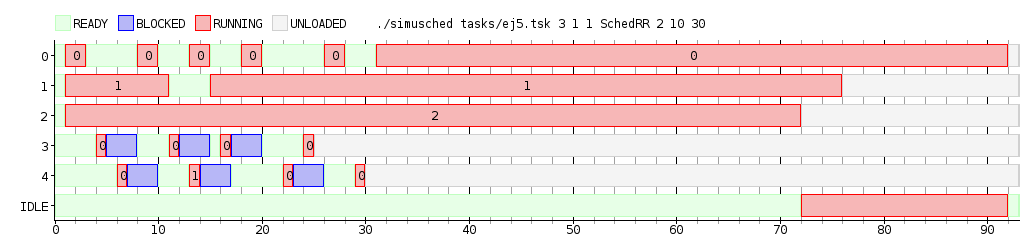
\includegraphics[width=1\columnwidth]{imagenes/ej5.png}
		\caption{\texttt{SchedRR} corriendo con tres núcleos: uno de quantum 2, 10 y otro de 30.}
		\label{fig:ej1_3n}
	\end{center}
\end{figure}

A continuación, se presentan los resultados de haber fijado la cantidad de núcleos
a 1 con un cambio de contexto de 2 ciclos variando únicamente el quantum para ver
así el efecto sobre la \emph{latencia}, \emph{waiting-time} y \emph{turnaround}
(tiempo total) promedio de las tareas descritas al comienzo del ejercicio.

\begin{figure}[H]
	\begin{center}
		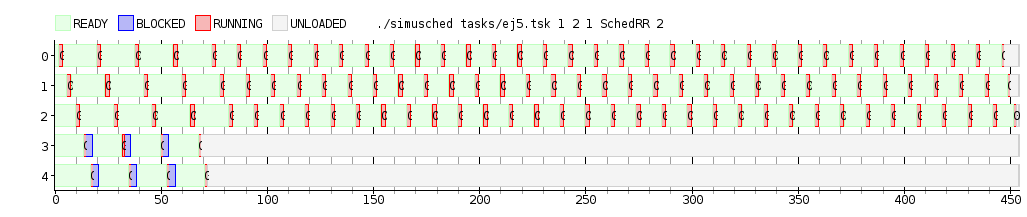
\includegraphics[width=1\columnwidth]{imagenes/ej5_q2.png}
		\caption{\texttt{SchedRR} corriendo con un núcleo de quantum 2}
	\end{center}
\end{figure}

\begin{figure}[H]
	\begin{center}
		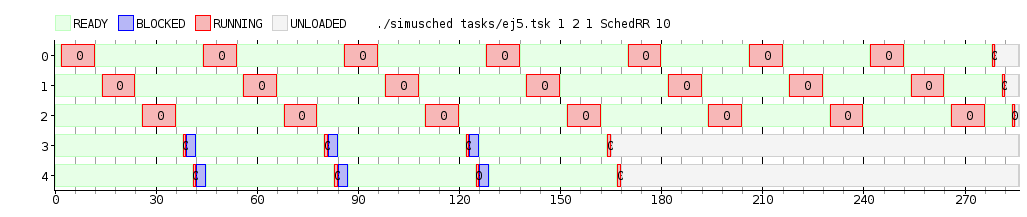
\includegraphics[width=1\columnwidth]{imagenes/ej5_q10.png}
		\caption{\texttt{SchedRR} corriendo con un núcleo de quantum 10}
	\end{center}
\end{figure}

\begin{figure}[H]
	\begin{center}
		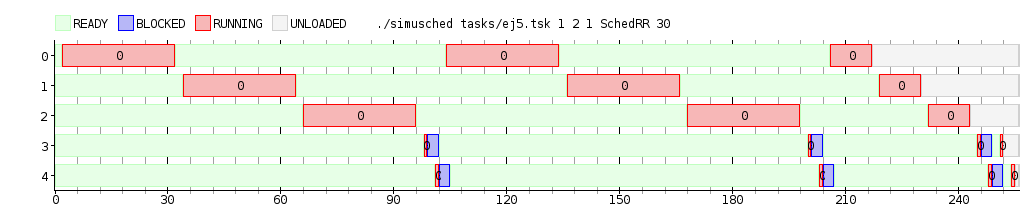
\includegraphics[width=1\columnwidth]{imagenes/ej5_q30.png}
		\caption{\texttt{SchedRR} corriendo con un núcleo de quantum 30}
	\end{center}
\end{figure}

Tomando los resultados anteriores se generó la siguiente tabla comparando los
tiempos para cada tamaño de quantum seleccionado.

\begin{figure}[H]
	\begin{center}
		\begin{tabular}{|c|c|c|c|}
			\hline
			\textbf{Quantum} & \textbf{Latencia} & \textbf{Waiting-time} & \textbf{Turnaround} \\ \hline
			2 & 9,8 & 250,4 & 298,2 \\ \hline
			10 & 24,2 & 188 & 235,8 \\ \hline
			30 & 60,2 & 191,6 & 239,4 \\ \hline
		\end{tabular}
		\caption{Tiempos promedio en función del tamaño de quantum utilizado}
	\end{center}
\end{figure}

A partir de esta información se pudieron desarrollar las siguiente conclusiones.
Para empezar, a simple vista se puede observar que ninguno de los tres tamaños
seleccionados es mejor en todos los criterios utilizados en simultáneo, esto
pone en evidencia el hecho de no existe una receta para todos los problemas, si
no que dependiendo las necesidades de uno, se debe decidir por alguno u otro.
Habiendo dicho esto, se pasan a describir los puntos fuertes y débiles de cada
quantum utilizado.

Para el quantum de \textbf{2}, la \emph{latencia} es la más baja con una amplia
diferencia respecto al resto. Esto es particularmente importante si se tienen
tareas interactivas donde se espera que el tiempo de respuesta sea alto. Sin
embargo, aquí se tiene que el \emph{waiting-time} y \emph{turnaround} son los
más altos de la tabla, indicando que en caso de tener tareas pesadas que
necesiten más tiempo del CPU este quantum no sería el apropiado.

Con un quantum de \textbf{10}, los resultados son bastante balanceados. La
\emph{latencia} es mejor que la del quantum de 30 pero peor que la de 2. Esto
tiene sentido ya que al aumentar el tamaño del quantum las tareas tienen que
esperar más a que termine su predecesor. Sin embargo, el \emph{waiting-time} es
el mejor de la tabla, y aquí es donde probablemente se deba a que con un quantum
de 10 se consigue el punto medio necesario para el lote de tareas generado, si
fuera muy pequeño, las tareas grandes desperdiciarían mucho tiempo
realizando cambio de contexto, si fuera grande, las tareas pequeñas deberían
esperar mucho para poder completarse.

Finalmente, fijando un quantum de \textbf{30}, se consiguen tiempos que son
ligeramente peores que los obtenidos por el de 10. En lo que es \emph{latencia},
es el peor de los tres, lo cual no es sorpresa ya que las primeras tareas en
ejecutarse son las de mayor consumo de CPU, dejando sin atender a las
bloqueantes. El \emph{waiting-time} es mejor que el de 2 pero levemente peor que
con 10, nuevamente debido al hecho de que al otrogarle más tiempo de
cómputo a las tareas intensivas, el resto espera más. Por último, el
\emph{turnaround}, que en principio uno podría suponer que sería el mejor (dado
que es el caso donde las tareas finalizan en menor tiempo) es también un
poco mayor que la de 10. Esto ocurre porque más allá de que finalicen antes que
el resto, el promedio es peor, ya que cuando se utilizaba un quantum de 10, las
tareas bloqueantes finalizaban antes.
